
\de{ĐỀ THI GIỮA HỌC KỲ I NĂM HỌC 2022-2023}{THPT Lê Quí Đôn}


\begin{bt}%[Dự án đề kiểm tra GHKI NH22-23- Ngô Quang Anh]%[0T4B2-1]
Cho tam giác $ABC$ có $AB=5$, $AC=8$ và $BC=9$.
	\begin{enumerate}[a)]
		\item Tính côsin của góc $B$ của tam giác $ABC$.
		\item Gọi $M$ là trung điểm của $BC$. Tính độ dài của đoạn $AM$.
	\end{enumerate}
\loigiai{
\begin{enumerate}[a)]
		\item Áp dụng hệ quả của định lí côsin, ta có
    \[\cos B =\dfrac{BC^2+AB^2-AC^2}{2BC\cdot AB}=\dfrac{9^2+5^2-8^2}{2\cdot 9 \cdot 5}=\dfrac{7}{15}.\]
   		\item Ta có $AM$ là đường trung tuyến của tam giác $ABC$. 
   		\[AM^2=\dfrac{AB^2+AC^2}{2}-\dfrac{BC^2}{4}=\dfrac{5^2+8^2}{2}-\dfrac{9^2}{4}=\dfrac{97}{4}\Leftrightarrow AM=\dfrac{\sqrt{97}}{2}.\]
\end{enumerate} 
    
}
\end{bt}
\begin{bt}%[Dự án đề kiểm tra GHKI NH22-23- Ngô Quang Anh]%[0T4B2-1]
Cho tam giác $ABC$ nội tiếp đường tròn bán kính $R$, $A B=R$, $AC=R\sqrt{3}$. Tính $\widehat{A}$ và tỉ số $\dfrac{R}{BC}$ biết $\widehat{B}$ là góc tù.
\loigiai{
Theo định lí hàm sin ta có 
\[\dfrac{AB}{\sin C}=\dfrac{AC}{\sin B}=\dfrac{BC}{\sin A}=2R\Rightarrow \dfrac{R}{\sin C}=\dfrac{R\sqrt{3}}{\sin B}=2R \Rightarrow \heva{&\sin C=\dfrac{1}{2}\\&\sin B=\dfrac{\sqrt{3}}{2}\\&\sin A=\dfrac{BC}{2R}.} \]
Mà $\widehat{B}$ là góc tù nên $ \heva{&\widehat{B}=120^\circ\\&\widehat{C}=30^\circ.} $\\
Suy ra $\widehat{A}=180^\circ-120^\circ-30^\circ=30^\circ$.\\
Ta có $\dfrac{R}{BC}=\dfrac{1}{2\sin A}=\dfrac{1}{2\sin 30^\circ}=1$.
}
\end{bt}
\begin{bt}%[Dự án đề kiểm tra GHKI NH22-23- Ngô Quang Anh]%[0T4B3-1]
Cho tam giác $ABC$ có $a=15$, $b=13$ và $c=14$. Tính:
	\begin{enumerate}[a)]
		\item Diện tích tam giác $ABC$.
		\item Bán kính đường tròn ngoại tiếp tam giác $ABC$.
	\end{enumerate}
\loigiai{
\begin{enumerate}[a)]
				\item Ta có $p=\dfrac{1}{2}(15+13+14)=21$.\\
				Áp dụng công thức Heron, ta có \[S=\sqrt{p(p-a)(p-b)(p-c)}=\sqrt{21(21-15)(21-13)(21-14)}=84.\]
				\item Ta có $S=\dfrac{abc}{4R}$, suy ra $R=\dfrac{abc}{4S}=\dfrac{15\cdot 13\cdot 14}{4\cdot 84}=\dfrac{65}{8}$.
			\end{enumerate}
}
\end{bt}
\begin{bt}%[Dự án đề kiểm tra GHKI NH22-23- Ngô Quang Anh]%[0T4K3-1]
Cho tam giác $ABC$ có cạnh $AB=14$, $\widehat{C}=120^{\circ}$, tổng hai cạnh còn lại là $16$. Tính độ dài hai cạnh còn lại, biết $BC>AC$.
\loigiai{
Theo giả thiết ta có $ CB+CA=16\Rightarrow CA=16-CB $.\\
Áp dụng hệ quả của định lí côsin, ta có
\allowdisplaybreaks
\begin{eqnarray*}
 &&\cos C =\dfrac{CA^2+CB^2-AB^2}{2CA\cdot CB}=-\dfrac{1}{2}\\
 &\Leftrightarrow& \dfrac{(16-CB)^2+CB^2-14^2}{2(16-CB)\cdot CB}=-\dfrac{1}{2}\\
 &\Leftrightarrow& CB^2-16CB+60=0\\
 &\Leftrightarrow& \hoac{&CB=10\Rightarrow AC=6&\text{ (nhận, vì } BC>AC\text{)}&\\&CB=6\Rightarrow AC=10&\text{ (loại)}&.}
\end{eqnarray*}
Vậy $CB=10$, $AC=6$.
}
\end{bt}
\begin{bt}%[Dự án đề kiểm tra GHKI NH22-23- Ngô Quang Anh]%[0T4K3-1]
\immini{Một tháp nước cao $30$ m ở trên đỉnh của một ngọn đồi. Từ tháp đến chân ngọn đồi dài $120$ m và người ta quan sát thấy góc tạo thành giữa đỉnh và chân tháp là $8^{\circ}$. Hỏi góc nghiêng của ngọn đồi so với phương ngang là bao nhiêu? (Kết quả được làm tròn đến độ).}
{
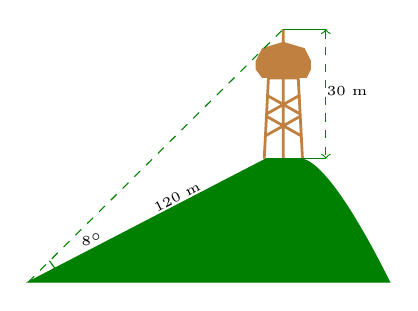
\begin{tikzpicture}
%\clip (-12.5,-10) rectangle (5,1.5);
%\begin{pgfinterruptboundingbox}
\tikzset{thap_nuoc/.pic={
\def\D{ % mái 
(-1,-.4)--(-1.3,0)--(-1.3,.4)--(-1,1)--(0,1.3)--(1,1)--(1.3,.4)--(1.3,0)--(1.1,-.4)--cycle
;}
%\draw[black] \D;
\fill[brown] \D;
%------------------chân tháp
\draw[color=brown, line width=1] (-.9,-4.2)--(-.7,-.4)--(.7,-.4)--(.9,-4.2)
(0,-.4)--(0,-4.2) (0,1.2)--(0,1.9)
(-.8,-1.2)--(.8,-2.1) (-.8,-2.1)--(.8,-1.2)
(-.8,-2.2)--(.8,-3.1) (-.8,-3.1)--(.8,-2.2)
;
\def\G{ % đồi
(-12,-10)--(-.8,-4.2)--(.8,-4.2)
..controls +(-5:1.5) and +(140:0.05) ..(5,-10)
--cycle
(-11,-9)--(-10.5,-9.7)
;}
\draw[green!50!black] \G;

\fill[color=green!50!black] \G;
\draw[dashed,green!50!black] (-12,-10)--(0,1.9);
\draw[dashed,green!50!black,<->] (2,1.9)--(2,-4.2);
\draw[green!50!black] (0,1.9)--(2,1.9)(0,-4.2)--(2,-4.2);
\node[rotate=27] at (-5,-6){\tiny $ 120 $ m};
\node at (-9,-8){\tiny $ 8^\circ $};
\node at (3,-1){\tiny $ 30 $ m};
}}
\path(0,0)pic[scale=.27]{thap_nuoc};
\end{tikzpicture}
}
\loigiai{
\immini{
Theo định lí hàm sin ta có 
\[\dfrac{BC}{\sin \widehat{BAC}}=\dfrac{AC}{\sin \widehat{ABC}}\Leftrightarrow \dfrac{30}{\sin 8^\circ}=\dfrac{120}{\sin \widehat{ABC}}\Rightarrow \sin \widehat{ABC}\approx 0{,}56\Rightarrow \widehat{ABC}\approx 34^\circ .\]
Suy ra $ \widehat{BAH}\approx 90^\circ - 34^\circ =56^\circ $.\\
Vậy góc nghiêng của ngọn đồi so với phương ngang là \[ \widehat{CAH}\approx 56^\circ -8^\circ =48^\circ.\]
}
{
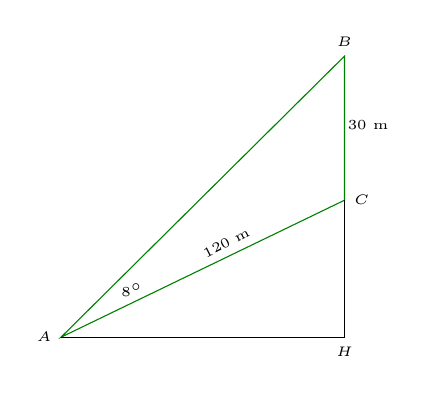
\begin{tikzpicture}[scale=.3]
\draw[green!50!black] (-12,-10)--(0,1.9)--(0,-4.2)--cycle;
\draw[black] (-12,-10)--(0,-10)--(0,-4.2);
\node[rotate=27] at (-5,-6){\tiny $ 120 $ m};

\node at (-9,-8){\tiny $ 8^\circ $};
\node at (1,-1){\tiny $ 30 $ m};
\node[left] at (-12,-10) {\tiny $ A $};
\node[above] at (0,1.9){\tiny $ B $};
\node[right] at (0,-4.2){\tiny $ C $};
\node[below] at (0,-10){\tiny $ H $};
\end{tikzpicture}
}
}
\end{bt}


